% ============================================================
%  presentation.tex — Thesis Defense Slides
%  PLAN STANDARD DE PRÉSENTATION — SOUTENANCE DE MÉMOIRE
%  AI-Driven Customer Intelligence & Sales Forecasting
%  ENSSEA 2025-2026 | Cherfaoui Houssam Abderrahmane
% ============================================================
\documentclass[aspectratio=169,12pt]{beamer}

% ── Encoding & Fonts ────────────────────────────────────────
\usepackage[utf8]{inputenc}
\usepackage[T1]{fontenc}
\usepackage{lmodern}
\usepackage{helvet}
\renewcommand{\familydefault}{\sfdefault}

% ── Packages ────────────────────────────────────────────────
\usepackage{graphicx}
\usepackage{booktabs}
\usepackage{array}
\usepackage{xcolor}
\usepackage{tikz}
\usepackage{pgfplots}
\pgfplotsset{compat=1.18}
\usepackage{amsmath}
\usepackage{multicol}
\usetikzlibrary{arrows.meta,positioning,shapes.geometric}

% ── Figures path ────────────────────────────────────────────
\graphicspath{{figures/}{titleimages/}}

% ── Colour Palette ──────────────────────────────────────────
\definecolor{PumaRed}    {HTML}{CC0000}
\definecolor{DarkBG}     {HTML}{121212}
\definecolor{CardBG}     {HTML}{1E1E1E}
\definecolor{PanelBG}    {HTML}{252525}
\definecolor{LightText}  {HTML}{F0F0F0}
\definecolor{MutedText}  {HTML}{AAAAAA}
\definecolor{GreenAccent}{HTML}{2ecc71}
\definecolor{BlueAccent} {HTML}{3498db}
\definecolor{OrangeAcc}  {HTML}{e67e22}

% ── Beamer Theme Setup ──────────────────────────────────────
\usetheme{default}
\setbeamertemplate{navigation symbols}{}
\setbeamertemplate{itemize item}{\color{PumaRed}\textbullet}
\setbeamertemplate{itemize subitem}{\color{MutedText}--}
\setbeamertemplate{enumerate item}{\color{PumaRed}\insertenumlabel.}

% Background
\setbeamercolor{background canvas}{bg=DarkBG}
\setbeamercolor{normal text}{fg=LightText,bg=DarkBG}
\setbeamercolor{alerted text}{fg=PumaRed}
\setbeamercolor{structure}{fg=PumaRed}

% Frame title
\setbeamercolor{frametitle}{fg=LightText,bg=CardBG}
\setbeamertemplate{frametitle}{%
  \vspace{0pt}%
  \begin{beamercolorbox}[wd=\paperwidth,ht=0.55cm,dp=0.2cm,leftskip=0.4cm]{frametitle}%
    {\color{PumaRed}\rule[-2pt]{3pt}{14pt}}\hspace{6pt}%
    \usebeamerfont{frametitle}\insertframetitle%
  \end{beamercolorbox}%
  \vspace{-2pt}%
  {\color{PumaRed}\rule{\linewidth}{0.4pt}}%
}

% Footer
\setbeamertemplate{footline}{%
  \begin{beamercolorbox}[wd=\paperwidth,ht=0.4cm,dp=0.15cm]{footline}%
    \color{MutedText}\hspace{0.3cm}{\tiny Cherfaoui H.A. | ENSSEA 2025--2026 | AI-Driven Customer Intelligence}%
    \hfill%
    {\tiny \insertframenumber\,/\,\inserttotalframenumber\hspace{0.3cm}}%
  \end{beamercolorbox}%
}

% Block colours
\setbeamercolor{block title}{bg=PanelBG,fg=PumaRed}
\setbeamercolor{block body} {bg=PanelBG,fg=LightText}

% ── Helper commands ──────────────────────────────────────────
\newcommand{\confirmed}{{\color{GreenAccent}\textbf{\checkmark\ Confirmed}}}
\newcommand{\metricbox}[2]{%
  \begin{tikzpicture}
    \node[fill=PanelBG,rounded corners=4pt,inner sep=8pt,
          draw=PumaRed,line width=0.6pt] {%
      \begin{tabular}{c}
        {\color{PumaRed}\large\textbf{#1}}\\[-2pt]
        {\color{MutedText}\scriptsize #2}
      \end{tabular}%
    };
  \end{tikzpicture}%
}
\newcommand{\panelbox}[1]{%
  \begin{tikzpicture}
    \node[fill=PanelBG,rounded corners=4pt,inner sep=10pt,
          draw=PumaRed,line width=0.5pt,text width=\linewidth-24pt]{#1};
  \end{tikzpicture}%
}

% ══════════════════════════════════════════════════════════════
%  DOCUMENT
% ══════════════════════════════════════════════════════════════
\begin{document}

% ─────────────────────────────────────────────────────────────
%  SLIDE 1 — PAGE DE TITRE
% ─────────────────────────────────────────────────────────────
\begin{frame}[plain]
\begin{tikzpicture}[remember picture, overlay]
  \fill[DarkBG] (current page.south west) rectangle (current page.north east);
  \fill[PumaRed] (current page.south west) rectangle
        ([xshift=0.18\paperwidth]current page.north west);
  \node[anchor=center] at ([xshift=0.09\paperwidth,yshift=0.10\paperheight]
        current page.south west) {%
    
\includegraphics[width=1.8cm]{Enssea.png}};
  \node[anchor=center,rotate=90,text width=5cm,align=center,
        font=\tiny\color{white}] at
        ([xshift=0.09\paperwidth,yshift=0.58\paperheight]
        current page.south west) {%
    \textbf{ENSSEA --- Kol\'ea, Algeria}};
  % Title
  \node[anchor=west,text width=0.74\paperwidth] at
        ([xshift=0.22\paperwidth,yshift=0.66\paperheight]
        current page.south west) {%
    {\color{LightText}\Large\bfseries AI-Driven Customer Intelligence}\\[4pt]
    {\color{LightText}\Large\bfseries \& Sales Forecasting}\\[10pt]
    {\color{PumaRed}\rule{9cm}{1.5pt}}\\[8pt]
    {\color{MutedText}\normalsize Segmentation $\cdot$ Customer Lifetime Value $\cdot$ Sales Prediction}\\[5pt]
    {\color{MutedText}\small\textit{Case Study: SARL GREAT WAY / PUMA Algeria}}%
  };
  % Author / Supervisor block
  \node[anchor=west,text width=0.74\paperwidth] at
        ([xshift=0.22\paperwidth,yshift=0.36\paperheight]
        current page.south west) {%
    \begin{tikzpicture}
      \node[fill=PanelBG,rounded corners=4pt,inner sep=10pt,
            draw=PumaRed,line width=0.5pt,text width=10cm]{%
        \begin{tabular}{ll}
          {\color{MutedText}\scriptsize Submitted by:}   & {\color{LightText}\small\bfseries Cherfaoui Houssam Abderrahmane}\\[4pt]
          {\color{MutedText}\scriptsize Supervised by:}  & {\color{LightText}\small Dr.\ Missi Sabrina --- Associate Professor}\\[4pt]
          {\color{MutedText}\scriptsize Degree:}         & {\color{LightText}\small Master in Statistics \& Applied Economics --- Data Science}\\[4pt]
          {\color{MutedText}\scriptsize Institution:}    & {\color{LightText}\small ENSSEA --- Kol\'ea, Algeria --- June 2026}\\
        \end{tabular}%
      };
    \end{tikzpicture}%
  };
\end{tikzpicture}
\end{frame}

% ─────────────────────────────────────────────────────────────
%  SLIDE 2 — STRUCTURE DU MÉMOIRE (ORGANIGRAMME)
% ─────────────────────────────────────────────────────────────
\begin{frame}{Thesis Structure}
\begin{center}

\begin{tikzpicture}
  \node[fill=CardBG,draw=PumaRed,rounded corners=4pt,inner sep=5pt,
        text=PumaRed,font=\scriptsize\bfseries,text width=5cm,align=center]
  {General Introduction};
\end{tikzpicture}
\end{center}
{\color{PumaRed}\rule{\linewidth}{0.4pt}}
\begin{columns}[t]
\column{0.32\textwidth}

\begin{tikzpicture}
  \node[fill=CardBG,draw=PumaRed,line width=1pt,rounded corners=4pt,
        inner sep=4pt,text=PumaRed,font=\scriptsize\bfseries,
        text width=3.5cm,align=center]
  {Chapter 1\\[1pt]Theoretical Foundations};
\end{tikzpicture}\\[2pt]
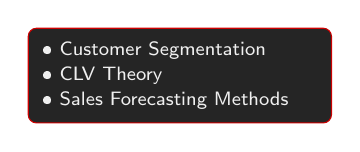
\begin{tikzpicture}
  \node[fill=PanelBG,draw=PumaRed,rounded corners=3pt,inner sep=5pt,
        text=LightText,font=\scriptsize,text width=3.5cm,align=left]{%
    \textbullet\ Customer Segmentation\\[1pt]
    \textbullet\ CLV Theory\\[1pt]
    \textbullet\ Sales Forecasting Methods};
\end{tikzpicture}

\column{0.32\textwidth}

\begin{tikzpicture}
  \node[fill=CardBG,draw=PumaRed,line width=1pt,rounded corners=4pt,
        inner sep=4pt,text=PumaRed,font=\scriptsize\bfseries,
        text width=3.5cm,align=center]
  {Chapter 2\\[1pt]Literature Review \&\\Company Framework};
\end{tikzpicture}\\[2pt]
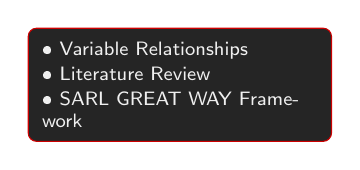
\begin{tikzpicture}
  \node[fill=PanelBG,draw=PumaRed,rounded corners=3pt,inner sep=5pt,
        text=LightText,font=\scriptsize,text width=3.5cm,align=left]{%
    \textbullet\ Variable Relationships\\[1pt]
    \textbullet\ Literature Review\\[1pt]
    \textbullet\ SARL GREAT WAY Framework};
\end{tikzpicture}

\column{0.32\textwidth}
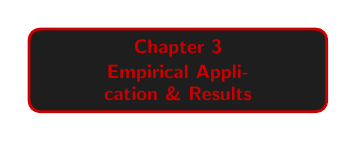
\begin{tikzpicture}
  \node[fill=CardBG,draw=PumaRed,line width=1pt,rounded corners=4pt,
        inner sep=4pt,text=PumaRed,font=\scriptsize\bfseries,
        text width=3.5cm,align=center]
  {Chapter 3\\[1pt]Empirical Application \& Results};
\end{tikzpicture}\\[2pt]
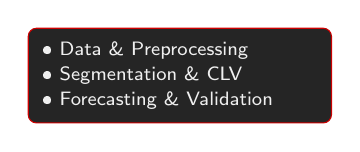
\begin{tikzpicture}
  \node[fill=PanelBG,draw=PumaRed,rounded corners=3pt,inner sep=5pt,
        text=LightText,font=\scriptsize,text width=3.5cm,align=left]{%
    \textbullet\ Data \& Preprocessing\\[1pt]
    \textbullet\ Segmentation \& CLV\\[1pt]
    \textbullet\ Forecasting \& Validation};
\end{tikzpicture}
\end{columns}
{\color{PumaRed}\rule{\linewidth}{0.4pt}}
\begin{center}

\begin{tikzpicture}
  \node[fill=CardBG,draw=PumaRed,rounded corners=4pt,inner sep=5pt,
        text=PumaRed,font=\scriptsize\bfseries,text width=5cm,align=center]
  {General Conclusion};
\end{tikzpicture}
\end{center}
\end{frame}

% ─────────────────────────────────────────────────────────────
%  SLIDE 3 — STRUCTURE DU MÉMOIRE (CONTENU)
% ─────────────────────────────────────────────────────────────
\begin{frame}{Chapter Contents}
\vspace{2pt}
\begin{columns}[t]
\column{0.33\textwidth}
  \textbf{\color{PumaRed}\small Chapter 1}\\
  {\color{MutedText}\scriptsize Theoretical Foundations}\\[4pt]
  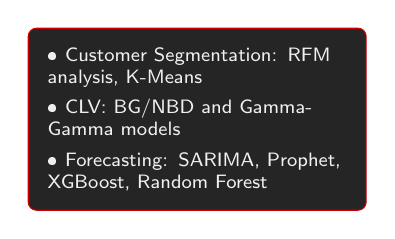
\begin{tikzpicture}
    \node[fill=PanelBG,draw=PumaRed,rounded corners=3pt,inner sep=7pt,
          text=LightText,font=\scriptsize,text width=3.8cm]{%
      \textbullet\ Customer Segmentation: RFM analysis, K-Means\\[3pt]
      \textbullet\ CLV: BG/NBD and Gamma-Gamma models\\[3pt]
      \textbullet\ Forecasting: SARIMA, Prophet, XGBoost, Random Forest
    };
  \end{tikzpicture}

\column{0.33\textwidth}
  \textbf{\color{PumaRed}\small Chapter 2}\\
  {\color{MutedText}\scriptsize Literature Review \& Framework}\\[4pt]
  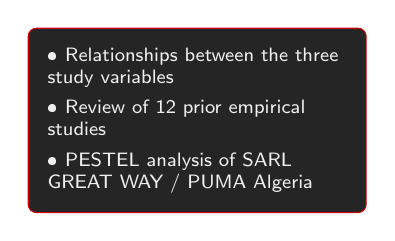
\begin{tikzpicture}
    \node[fill=PanelBG,draw=PumaRed,rounded corners=3pt,inner sep=7pt,
          text=LightText,font=\scriptsize,text width=3.8cm]{%
      \textbullet\ Relationships between the three study variables\\[3pt]
      \textbullet\ Review of 12 prior empirical studies\\[3pt]
      \textbullet\ PESTEL analysis of SARL GREAT WAY / PUMA Algeria
    };
  \end{tikzpicture}

\column{0.33\textwidth}
  \textbf{\color{PumaRed}\small Chapter 3}\\
  {\color{MutedText}\scriptsize Empirical Application}\\[4pt]
  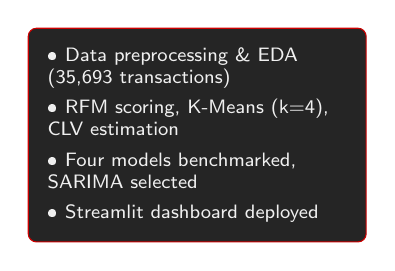
\begin{tikzpicture}
    \node[fill=PanelBG,draw=PumaRed,rounded corners=3pt,inner sep=7pt,
          text=LightText,font=\scriptsize,text width=3.8cm]{%
      \textbullet\ Data preprocessing \& EDA (35,693 transactions)\\[3pt]
      \textbullet\ RFM scoring, K-Means (k=4), CLV estimation\\[3pt]
      \textbullet\ Four models benchmarked, SARIMA selected\\[3pt]
      \textbullet\ Streamlit dashboard deployed
    };
  \end{tikzpicture}
\end{columns}
\end{frame}

% ─────────────────────────────────────────────────────────────
%  SLIDE 4 — INTRODUCTION ET PROBLÉMATIQUE
% ─────────────────────────────────────────────────────────────
\begin{frame}{Introduction \& Research Problem}
\begin{columns}[t]
\column{0.48\textwidth}
  \textbf{\color{PumaRed}\small General Context}\\[2pt]
  {\scriptsize Retail companies accumulate large transaction data but rarely transform it into decisions. SARL GREAT WAY --- exclusive PUMA distributor across \textbf{13 boutiques in Algeria} --- had full ERP data but no analytical pipeline to exploit it.}\\[4pt]

  \textbf{\color{PumaRed}\small Research Problem}\\[2pt]
  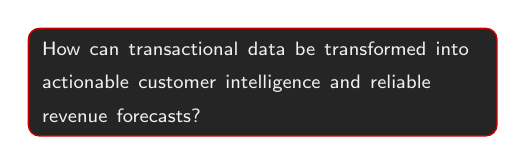
\begin{tikzpicture}
    \node[fill=PanelBG,rounded corners=4pt,inner sep=5pt,
          draw=PumaRed,line width=0.5pt,text width=5.6cm]{%
      {\color{LightText}\scriptsize How can transactional data be transformed into actionable customer intelligence and reliable revenue forecasts?}
    };
  \end{tikzpicture}

\column{0.50\textwidth}
  \textbf{\color{PumaRed}\small Three Specific Objectives}
  \begin{enumerate}\scriptsize
    \item Segment customers by purchasing behaviour: RFM + K-Means
    \item Estimate CLV using BG/NBD and Gamma-Gamma models
    \item Build and compare four forecasting models: SARIMA, Prophet, XGBoost, RF
  \end{enumerate}
  \vspace{2pt}
  \textbf{\color{PumaRed}\small Five Research Hypotheses}
  \begin{itemize}\scriptsize
    \item[\color{PumaRed}\textbf{H1}] K-Means produces statistically distinct segments
    \item[\color{PumaRed}\textbf{H2}] BG/NBD accurately predicts repeat purchases
    \item[\color{PumaRed}\textbf{H3}] Gamma-Gamma reliably estimates transaction value
    \item[\color{PumaRed}\textbf{H4}] At least one model achieves error below 20\%
    \item[\color{PumaRed}\textbf{H5}] Top 20\% customers hold disproportionate CLV (Pareto)
  \end{itemize}
\end{columns}
\end{frame}

% ─────────────────────────────────────────────────────────────
%  SLIDE 5 — REVUE DE LITTÉRATURE
% ─────────────────────────────────────────────────────────────
\begin{frame}{Literature Review --- State of the Art}
{\color{PumaRed}\rule{\linewidth}{0.4pt}}
\centering\vspace{1pt}
{\scriptsize
\begin{tabular}{p{2.8cm}p{2.5cm}p{6.0cm}}
  \toprule
  \textbf{\color{LightText}Authors} & \textbf{\color{LightText}Method} & \textbf{\color{LightText}Key Contribution}\\
  \midrule
  Hughes (1996)               & RFM Scoring     & Quintile-based customer scoring\\[1pt]
  Schmittlein et al.\ (1987)  & Pareto/NBD      & First probabilistic CLV model\\[1pt]
  Fader et al.\ (2005)        & BG/NBD          & Tractable CLV for non-contractual settings\\[1pt]
  Fader \& Hardie (2013)      & Gamma-Gamma     & Monetary value estimation by Bayesian shrinkage\\[1pt]
  Tsiptsis et al.\ (2009)     & K-Means CRM     & Clustering for actionable CRM segmentation\\[1pt]
  Box \& Jenkins (1976)       & ARIMA/SARIMA    & Seasonal time series modelling\\[1pt]
  Taylor \& Letham (2018)     & Prophet         & Scalable additive decomposition forecasting\\[1pt]
  Chen \& Guestrin (2016)     & XGBoost         & Gradient boosting for regression tasks\\[1pt]
  Makridakis et al.\ (2018)   & M4 Competition  & SARIMA competitive against ML on short series\\
  \bottomrule
\end{tabular}
}
\vspace{2pt}
{\color{PumaRed}\rule{\linewidth}{0.4pt}}\vspace{2pt}

\raggedright
{\scriptsize{\color{PumaRed}\textbf{Research Gap:}}
{\color{MutedText} No integrated RFM + probabilistic CLV + multi-model forecasting pipeline applied to Algerian retail data.}}
\end{frame}

% ─────────────────────────────────────────────────────────────
%  SLIDE 6 — CADRE THÉORIQUE ET RELATIONS ENTRE VARIABLES
% ─────────────────────────────────────────────────────────────
\begin{frame}{Theoretical Framework --- Variable Relationships}
\begin{columns}[c]
\column{0.52\textwidth}
\centering
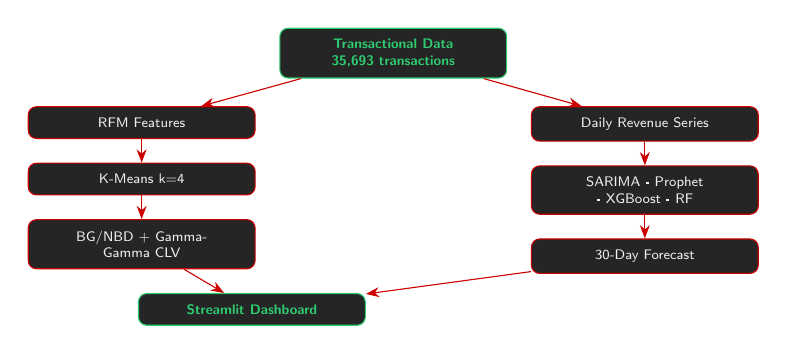
\begin{tikzpicture}[
  box/.style={fill=PanelBG,draw=PumaRed,rounded corners=3pt,
              text=LightText,font=\tiny,inner sep=4pt,text width=2.6cm,align=center},
  arr/.style={-Stealth,color=PumaRed}
]
  \node[box,draw=GreenAccent,text=GreenAccent,font=\tiny\bfseries] (data)
        {Transactional Data\\35,693 transactions};

  \node[box, below left=0.35cm and 0.3cm of data]  (rfm)   {RFM Features};
  \node[box, below right=0.35cm and 0.3cm of data] (ts)    {Daily Revenue Series};

  \node[box, below=0.3cm of rfm]  (kmeans) {K-Means k=4};
  \node[box, below=0.3cm of kmeans] (clv)  {BG/NBD + Gamma-Gamma CLV};

  \node[box, below=0.3cm of ts]   (models) {SARIMA · Prophet · XGBoost · RF};
  \node[box, below=0.3cm of models] (fc)   {30-Day Forecast};

  \node[box, draw=GreenAccent, below=0.3cm of clv,
        text=GreenAccent, font=\tiny\bfseries, text width=2.6cm, xshift=1.4cm]
        (dash) {Streamlit Dashboard};

  \draw[arr] (data)--(rfm); \draw[arr] (data)--(ts);
  \draw[arr] (rfm)--(kmeans); \draw[arr] (kmeans)--(clv);
  \draw[arr] (ts)--(models); \draw[arr] (models)--(fc);
  \draw[arr] (clv)--(dash); \draw[arr] (fc)--(dash);
\end{tikzpicture}

\column{0.46\textwidth}
  \textbf{\color{PumaRed}\small Key Theoretical Links}\\[3pt]
  \begin{itemize}\scriptsize
    \item \textbf{RFM $\to$ Segmentation:} behavioural features reveal loyalty profiles
    \item \textbf{Segmentation $\to$ CLV:} segment membership predicts future value
    \item \textbf{CLV $\to$ Forecasting:} high-CLV concentration explains revenue skew
    \item \textbf{Forecasting $\to$ Planning:} SARIMA cycle validates seasonal findings
  \end{itemize}
  \vspace{3pt}
  \textbf{\color{PumaRed}\small Conceptual Position}\\[2pt]
  {\scriptsize This study applies \textit{probabilistic non-contractual CLV theory} (Fader \& Hardie) and \textit{Box-Jenkins time series analysis} within a \textit{quantitative retail analytics} framework.}
\end{columns}
\end{frame}

% ─────────────────────────────────────────────────────────────
%  SLIDE 7 — MÉTHODOLOGIE : APPROCHE ET DONNÉES
% ─────────────────────────────────────────────────────────────
\begin{frame}{Methodology --- Research Approach \& Data}
\begin{columns}[t]
\column{0.42\textwidth}
  \textbf{\color{PumaRed}\small Approach \& Tools}
  \begin{itemize}\tiny
    \item \textbf{Type:} Quantitative empirical study
    \item \textbf{Source:} Real ERP data from SARL GREAT WAY
    \item \textbf{Tools:} Python 3.13 · lifetimes · pmdarima · prophet · xgboost · sklearn · Streamlit
    \item \textbf{Variables:} Date, Client ID, Revenue, Category
    \item \textbf{Cleaning:} Returns excluded, 97th-pct outlier clipping, gap-filling
  \end{itemize}

\column{0.56\textwidth}
  \centering
  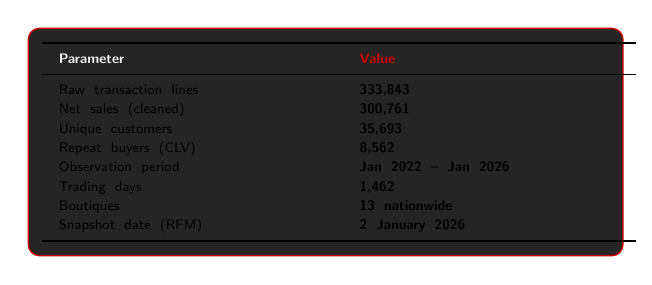
\begin{tikzpicture}
    \node[fill=PanelBG,rounded corners=4pt,inner sep=5pt,
          draw=PumaRed,line width=0.5pt,text width=7.2cm]{%
      \tiny
      \begin{tabular}{p{3.4cm}p{3.3cm}}
        \toprule
        \textbf{\color{LightText}Parameter} & \textbf{\color{PumaRed}Value}\\
        \midrule
        Raw transaction lines  & \textbf{333,843}\\[1pt]
        Net sales (cleaned)    & \textbf{300,761}\\[1pt]
        Unique customers       & \textbf{35,693}\\[1pt]
        Repeat buyers (CLV)    & \textbf{8,562}\\[1pt]
        Observation period     & \textbf{Jan 2022 -- Jan 2026}\\[1pt]
        Trading days           & \textbf{1,462}\\[1pt]
        Boutiques              & \textbf{13 nationwide}\\[1pt]
        Snapshot date (RFM)    & \textbf{2 January 2026}\\
        \bottomrule
      \end{tabular}%
    };
  \end{tikzpicture}
\end{columns}
\end{frame}

% ─────────────────────────────────────────────────────────────
%  SLIDE 8 — MÉTHODOLOGIE : PIPELINE ET LIMITES
% ─────────────────────────────────────────────────────────────
\begin{frame}{Methodology --- Analytical Pipeline \& Limits}
\begin{columns}[t]
\column{0.55\textwidth}
  \textbf{\color{PumaRed}\small Three-Stage Pipeline}\\[3pt]
  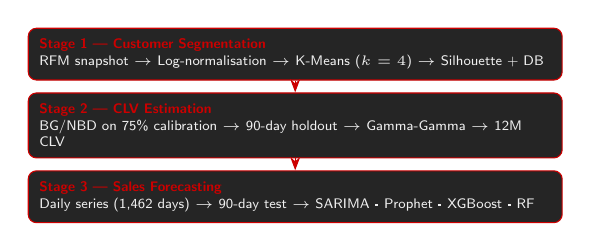
\begin{tikzpicture}[node distance=0.2cm,
    stage/.style={fill=PanelBG,draw=PumaRed,rounded corners=3pt,
                  text=LightText,font=\tiny,inner sep=4pt,text width=6.5cm},
    arr/.style={-Stealth,color=PumaRed}]
    \node[stage] (s1) {\textbf{\color{PumaRed}Stage 1 — Customer Segmentation}\\
      RFM snapshot $\to$ Log-normalisation $\to$ K-Means ($k=4$) $\to$ Silhouette + DB};
    \node[stage, below=0.15cm of s1] (s2) {\textbf{\color{PumaRed}Stage 2 — CLV Estimation}\\
      BG/NBD on 75\% calibration $\to$ 90-day holdout $\to$ Gamma-Gamma $\to$ 12M CLV};
    \node[stage, below=0.15cm of s2] (s3) {\textbf{\color{PumaRed}Stage 3 — Sales Forecasting}\\
      Daily series (1,462 days) $\to$ 90-day test $\to$ SARIMA · Prophet · XGBoost · RF};
    \draw[-Stealth,PumaRed] (s1)--(s2); \draw[-Stealth,PumaRed] (s2)--(s3);
  \end{tikzpicture}

\column{0.43\textwidth}
  \textbf{\color{PumaRed}\small Methodological Limits}\\[3pt]
  \begin{itemize}\scriptsize
    \item \textbf{CLV coverage:} 24\% only (repeat buyers)
    \item \textbf{Single split:} no rolling cross-validation
    \item \textbf{k=4 selection:} elbow + silhouette, no gap statistic
    \item \textbf{Discount rate:} approximated, not market-calibrated
    \item \textbf{Single company:} recalibration needed for other brands
  \end{itemize}
\end{columns}
\end{frame}

% ─────────────────────────────────────────────────────────────
%  SLIDE 9 — RÉSULTATS : SEGMENTATION
% ─────────────────────────────────────────────────────────────
\begin{frame}{Results --- Customer Segmentation}
\begin{columns}[c]
\column{0.50\textwidth}
  \centering
  \includegraphics[width=\linewidth,height=5.5cm,keepaspectratio]{fig_kmeans_radar.png}
  {\color{MutedText}\tiny Radar chart --- normalised K-Means segment centroids}

\column{0.48\textwidth}
  \centering
  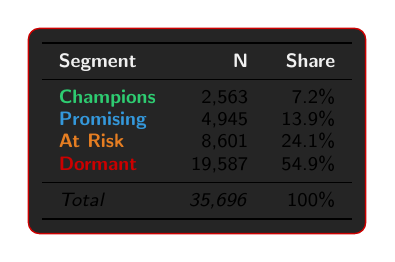
\begin{tikzpicture}
    \node[fill=PanelBG,rounded corners=4pt,inner sep=5pt,
          draw=PumaRed,line width=0.5pt]{%
      \scriptsize\begin{tabular}{lrr}
        \toprule
        \textbf{\color{LightText}Segment} & \textbf{\color{LightText}N} & \textbf{\color{LightText}Share}\\
        \midrule
        {\color{GreenAccent}\textbf{Champions}}    & 2,563  & 7.2\%\\
        {\color{BlueAccent}\textbf{Promising}}     & 4,945  & 13.9\%\\
        {\color{OrangeAcc}\textbf{At Risk}}        & 8,601  & 24.1\%\\
        {\color{PumaRed}\textbf{Dormant}}          & 19,587 & 54.9\%\\
        \midrule
        \textit{Total} & \textit{35,696} & 100\%\\
        \bottomrule
      \end{tabular}%
    };
  \end{tikzpicture}
  \vspace{3pt}
  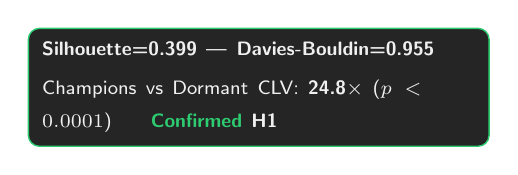
\begin{tikzpicture}
    \node[fill=PanelBG,rounded corners=4pt,inner sep=5pt,
          draw=GreenAccent,line width=0.5pt,text width=5.5cm]{%
      {\color{LightText}\scriptsize \textbf{Silhouette=0.399} | \textbf{Davies-Bouldin=0.955}\\[2pt]
      Champions vs Dormant CLV: \textbf{24.8$\times$} ($p<0.0001$) \quad \confirmed\ \textbf{H1}}
    };
  \end{tikzpicture}
\end{columns}
\end{frame}

% ─────────────────────────────────────────────────────────────
%  SLIDE 10 — RÉSULTATS : CLV
% ─────────────────────────────────────────────────────────────
\begin{frame}{Results --- Customer Lifetime Value}
\begin{columns}[c]
\column{0.50\textwidth}
  \centering
  \includegraphics[width=\linewidth,height=5cm,keepaspectratio]{fig_bgnbd_cohort.png}
  {\color{MutedText}\tiny BG/NBD holdout --- predicted vs actual by frequency cohort}

\column{0.48\textwidth}
  \textbf{\color{PumaRed}\small BG/NBD Validation (90-day holdout)}
  \begin{itemize}\scriptsize
    \item MAE = \textbf{0.279 transactions / customer}
    \item Predicted tracks actual for all cohorts F=1 to F=10
    \item \confirmed\ \textbf{H2}
  \end{itemize}
  \vspace{2pt}
  \textbf{\color{PumaRed}\small CLV Summary (12-month horizon)}
  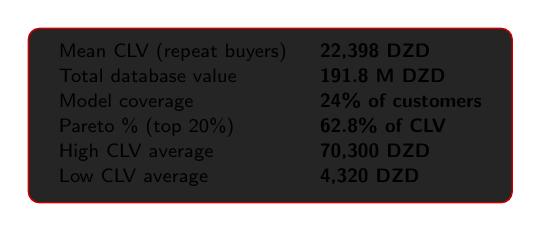
\begin{tikzpicture}
    \node[fill=PanelBG,rounded corners=4pt,inner sep=5pt,
          draw=PumaRed,line width=0.5pt]{%
      \scriptsize\begin{tabular}{ll}
        Mean CLV (repeat buyers) & \textbf{22,398 DZD}\\[1pt]
        Total database value     & \textbf{191.8 M DZD}\\[1pt]
        Model coverage           & \textbf{24\% of customers}\\[1pt]
        Pareto \% (top 20\%)     & \textbf{62.8\% of CLV}\\[1pt]
        High CLV average         & \textbf{70,300 DZD}\\[1pt]
        Low CLV average          & \textbf{4,320 DZD}\\
      \end{tabular}%
    };
  \end{tikzpicture}
  \vspace{2pt}
  {\scriptsize \confirmed\ \textbf{H3} \quad \confirmed\ \textbf{H5} (Pareto 62.8\%)}
\end{columns}
\end{frame}

% ─────────────────────────────────────────────────────────────
%  SLIDE 11 — RÉSULTATS : FORECASTING
% ─────────────────────────────────────────────────────────────
\begin{frame}{Results --- Sales Forecasting}
\begin{columns}[c]
\column{0.50\textwidth}
  \centering
  \includegraphics[width=\linewidth,height=5cm,keepaspectratio]{fig_actual_vs_pred.png}
  {\color{MutedText}\tiny Actual vs predicted daily revenue --- 90-day test window}

\column{0.48\textwidth}
  \textbf{\color{PumaRed}\small Model Ranking (MAE --- lower is better)}\\[2pt]
  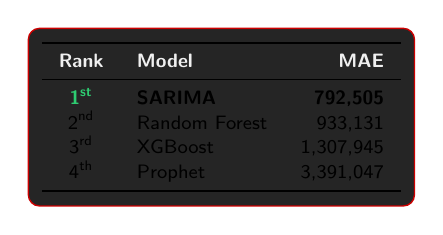
\begin{tikzpicture}
    \node[fill=PanelBG,rounded corners=4pt,inner sep=5pt,
          draw=PumaRed,line width=0.5pt]{%
      \scriptsize\begin{tabular}{clr}
        \toprule
        \textbf{\color{LightText}Rank} & \textbf{\color{LightText}Model} & \textbf{\color{LightText}MAE}\\
        \midrule
        {\color{GreenAccent}\textbf{1\textsuperscript{st}}} & \textbf{SARIMA} & \textbf{792,505}\\
        2\textsuperscript{nd} & Random Forest & 933,131\\
        3\textsuperscript{rd} & XGBoost       & 1,307,945\\
        4\textsuperscript{th} & Prophet       & 3,391,047\\
        \bottomrule
      \end{tabular}%
    };
  \end{tikzpicture}
  \vspace{2pt}
  \begin{itemize}\scriptsize
    \item SARIMA$(2,1,2)(1,0,1)_7$ via ACF/PACF
    \item Forecast Error = \textbf{18.6\%} ($<$ 20\% threshold)
    \item 30-day projection: \textbf{91.34 M DZD}
  \end{itemize}
  \vspace{2pt}
  {\scriptsize \confirmed\ \textbf{H4}}
\end{columns}
\end{frame}

% ─────────────────────────────────────────────────────────────
%  SLIDE 12 — DISCUSSION : COMPARAISON ET APPORTS
% ─────────────────────────────────────────────────────────────
\begin{frame}{Discussion --- Comparison with Literature \& Contributions}
\begin{columns}[t]
\column{0.50\textwidth}
  \textbf{\color{PumaRed}\small Concordance with Prior Studies}
  \begin{itemize}\scriptsize
    \item BG/NBD outperforms heuristics --- \textit{Fader et al.\ (2005)}
    \item K-Means on RFM produces actionable segments --- \textit{Tsiptsis et al.\ (2009)}
    \item SARIMA beats ML on short series --- \textit{Makridakis M4 (2018)}
    \item Pareto 62.8\% is below 80/20 but consistent with B2C retail
  \end{itemize}
  \vspace{2pt}
  \textbf{\color{PumaRed}\small Divergence}
  \begin{itemize}\scriptsize
    \item Prophet underperforms: insufficient data for yearly seasonality
  \end{itemize}

\column{0.48\textwidth}
  \textbf{\color{PumaRed}\small Theoretical Contributions}
  \begin{itemize}\scriptsize
    \item First integrated RFM + BG/NBD + multi-model forecasting pipeline on Algerian retail data
    \item Validates probabilistic CLV in a non-Western developing market
    \item SARIMA vs ML benchmark on the Algerian commercial calendar
  \end{itemize}
  \vspace{2pt}
  \textbf{\color{PumaRed}\small Practical Contributions}
  \begin{itemize}\scriptsize
    \item Streamlit dashboard for non-technical managers
    \item Five hypothesis-driven findings actionable for PUMA Algeria strategy
  \end{itemize}
\end{columns}
\end{frame}

% ─────────────────────────────────────────────────────────────
%  SLIDE 13 — DISCUSSION : LIMITES ET IMPLICATIONS
% ─────────────────────────────────────────────────────────────
\begin{frame}{Discussion --- Limits \& Implications}
\begin{columns}[t]
\column{0.50\textwidth}
  \textbf{\color{PumaRed}\small Study Limitations}\\[2pt]
  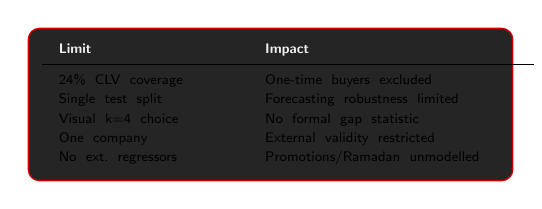
\begin{tikzpicture}
    \node[fill=PanelBG,rounded corners=4pt,inner sep=5pt,
          draw=PumaRed,line width=0.5pt,text width=5.8cm]{%
      \tiny
      \begin{tabular}{p{2.2cm}p{3.2cm}}
        \textbf{\color{LightText}Limit} & \textbf{\color{LightText}Impact}\\
        \midrule
        24\% CLV coverage & One-time buyers excluded\\[1pt]
        Single test split & Forecasting robustness limited\\[1pt]
        Visual k=4 choice & No formal gap statistic\\[1pt]
        One company       & External validity restricted\\[1pt]
        No ext.\ regressors & Promotions/Ramadan unmodelled\\
      \end{tabular}%
    };
  \end{tikzpicture}

\column{0.48\textwidth}
  \textbf{\color{PumaRed}\small Managerial Implications}
  \begin{itemize}\scriptsize
    \item \textbf{Champions (7.2\%):} VIP program, exclusive access
    \item \textbf{At Risk (24.1\%):} Win-back campaigns before churn
    \item \textbf{CLV scores:} Optimise acquisition vs retention budget
    \item \textbf{30-day forecast:} Inventory and staffing planning
  \end{itemize}
  \vspace{2pt}
  \textbf{\color{PumaRed}\small Academic Implications}
  \begin{itemize}\scriptsize
    \item Validates probabilistic CLV in developing market retail
    \item Confirms SARIMA competitive against ML on short retail series
  \end{itemize}
\end{columns}
\end{frame}

% ─────────────────────────────────────────────────────────────
%  SLIDE 14 — CONCLUSION GÉNÉRALE
% ─────────────────────────────────────────────────────────────
\begin{frame}{General Conclusion}
\vspace{-2pt}
% Hypothesis strip
\begin{center}
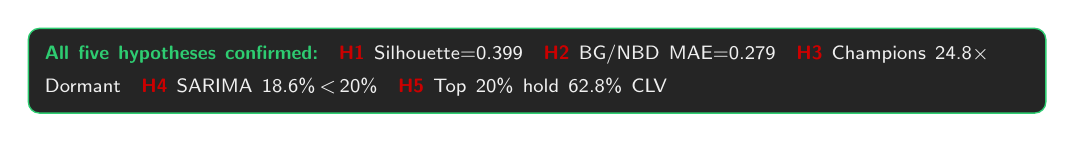
\begin{tikzpicture}
  \node[fill=PanelBG,draw=GreenAccent,rounded corners=4pt,inner sep=6pt,
        line width=0.5pt,text width=12.5cm]{%
    \scriptsize\color{LightText}
    \textbf{\color{GreenAccent}All five hypotheses confirmed:}\quad
    \textbf{\color{PumaRed}H1} Silhouette=0.399\quad
    \textbf{\color{PumaRed}H2} BG/NBD MAE=0.279\quad
    \textbf{\color{PumaRed}H3} Champions 24.8$\times$ Dormant\quad
    \textbf{\color{PumaRed}H4} SARIMA 18.6\%\,$<$\,20\%\quad
    \textbf{\color{PumaRed}H5} Top 20\% hold 62.8\% CLV\quad
    {\color{GreenAccent}\checkmark\checkmark\checkmark\checkmark\checkmark}
  };
\end{tikzpicture}
\end{center}
\vspace{4pt}
\begin{columns}[t]
\column{0.50\textwidth}
  \textbf{\color{PumaRed}\small Answer to Research Problem}\\[3pt]
  {\scriptsize Transactional data from SARL GREAT WAY can be transformed into actionable customer intelligence and reliable revenue forecasts through a validated three-stage pipeline, with results directly deployable for business decisions.}\\[5pt]

  \textbf{\color{PumaRed}\small Practical Output}\\[3pt]
  {\scriptsize An interactive Streamlit dashboard consolidating segmentation, CLV scores, and 30-day revenue projections — accessible to non-technical managers.}

\column{0.48\textwidth}
  \textbf{\color{PumaRed}\small Future Research}
  \begin{itemize}\scriptsize
    \item Add product diversity as a 4th RFM dimension
    \item Rolling CLV updates to track segment migration
    \item Second year of data for proper cross-validation
    \item External regressors: Ramadan, promotional events
    \item Extend pipeline to other PUMA distributors
  \end{itemize}
\end{columns}
\end{frame}

% ─────────────────────────────────────────────────────────────
%  SLIDE 15 — THANK YOU
% ─────────────────────────────────────────────────────────────
\begin{frame}[plain]
\begin{tikzpicture}[remember picture,overlay]
  \fill[DarkBG] (current page.south west) rectangle (current page.north east);
  \fill[PumaRed] (current page.south west) rectangle
        ([xshift=0.18\paperwidth]current page.north west);
  \node[anchor=center] at ([xshift=0.09\paperwidth]current page.center) {%
    
\includegraphics[width=1.8cm]{Enssea.png}};
  \node[anchor=west,text width=0.74\paperwidth] at
        ([xshift=0.22\paperwidth,yshift=0.14\paperheight]current page.center) {%
    {\color{MutedText}\small ENSSEA --- Kol\'ea, Algeria \quad|\quad June 2026}%
  };
  \node[anchor=west,text width=0.74\paperwidth] at
        ([xshift=0.22\paperwidth]current page.center) {%
    {\color{LightText}\Huge\bfseries Thank You}\\[10pt]
    {\color{PumaRed}\rule{9cm}{1.5pt}}\\[10pt]
    {\color{MutedText}\normalsize I am available for your questions.}%
  };
  \node[anchor=west,text width=0.74\paperwidth] at
        ([xshift=0.22\paperwidth,yshift=-0.18\paperheight]current page.center) {%
    {\color{MutedText}\scriptsize \textbf{Cherfaoui Houssam Abderrahmane}
     \quad|\quad Supervised by Dr.\ Missi Sabrina --- Associate Professor}%
  };
\end{tikzpicture}
\end{frame}

\end{document}
